\section{Methods}
We implemented a genetic solver in C++ using genetic algorithm with a local search improvement.
The data we used for benchmarks is in DIMACS CNF format, which is a formula in conjunction (logical and) of a set of clauses. And we decided to use the randomly generated 3-SAT-instances that are satisfiable in this format. 

A candidate solution is a string of bits whose length equals to the number of variables of the considered problem instance. To generate healthy population that could lead to the final solution, firstly we repeatedly generate random assignments for the instance until a certain number of population reached in the current generation. We use a population consists of 256 individuals. Then repeat actions on the whole candidate solutions: In each iteration, firstly select some best individuals. The fitness function we used to evaluate individuals is the number of satisfied clauses. Then crossover are performed on two individuals among the bests. Each generated child is improved individually using a local search process, and then new individuals are inserted and old individuals are removed in the population under some conditions. Iterate the process until a solution is generated, that is when the maximum number of satisfied clauses equals to the number of instance clauses. The general algorithm is illustrated in Fig\ref{fig:1.png}. 
\begin{figure}[h]
    \centering
    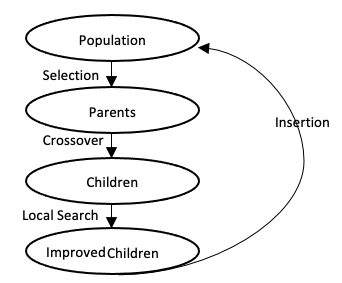
\includegraphics[width=0.4\textwidth]{1.png}
    \caption{Algorithm Scheme}
    \label{fig:1.png}
\end{figure}
\subsection{Selection Operation}
For selection, we adapt part of the idea of tournament selection, which has small algorithm complexity of O(n) (where n is the tournament size). We randomly select a certain number of individuals and then selected the top few individuals in descending order of fitness. The number of individuals randomly selected as tournament size is set to 16 and the number of best individuals among the tournament size is set to 4.
\subsection{Crossover Operators}
The main goal of the crossover operator in our genetic solver is to create potentially promising new individuals. Using the randomly selected a pair of parents from the resulting selected individuals from the tournament selection, there are many ways for them to crossover, and we consider 5 types: CC (Corrective Clause) Crossover, F\&F (Fleurent and Ferland) Crossover, Uniform Crossover, One-point Crossover and Two-point Crossover. We will introduce them respectively below.

CC (Corrective Clause) Crossover:
For each clause c that is unsatisfiable for both parent\_x and parent\_y solutions and for each variables that appears in clause c, find the bit position using the literally absolute value $i$ of the variable that produces the maximum improvement on two parents guided by the improvement evaluation function. The function equals to the number of false clauses which become true by flipping the $ith$ bit in one of the solutions minus the number of satisfied clauses which become false. Assign the flipped value applied to one of the parents to the child in the bit position found, and all the bits with no value of child take the value in corresponding position of parent\_x or parent\_y with the equal probability.

F\&F (Fleurent and Ferland) Crossover:
For each clause c that is satisfiable for one parent and unsatisfiable for the other parent and for each variables that appears in clause c, the bits positions in the child, corresponding to the literally absolute value $i$ of the variable in parents, are assigned values according to the parent satisfying the identified clause. All the bits with no value of the child take the value in corresponding position of parent\_x or parent\_y with the equal probability.

Uniform Crossover:
With equal probability, each bits of the child is chosen from either parent. In that case, one new offspring is generated.

One-point Crossover:
Randomly select one pivot point (ranging between 0 to length of the bits string) and exchange the substring from that bit point till the end of the string between the two individuals. In that case, two new offspring individual are generated.

Two-point Crossover:
Randomly pick two pivot points and the bits in between the two points are swapped between the parent individuals. In that case, two new offspring individual are generated.
% mutation operators.\\
\subsection{Local Search}
We implement the idea of mutation in genetic algorithm using WalkSat local search method. It's a randomized local search algorithm. It attempts to determine the best move by randomly choosing a clause among those that are currently unsatisfied and selecting a variable to flip within it under some conditions. The number of tries (Maxtries) is set to 1000. The search stops when one solution is found.

\subsection{Three Performance Measures}
After all these processes to generate a solution, we compare our solver using different crossovers and with other existing solvers. Several runs are required for each benchmark instance under consideration and some measuring methods need to be taken for statistically meaningful and also relatively fair results. We take 10 runs and consider three measuring methods: SR (Success rate), AT (Average Time) and AFS (Average Flips to Solution). We will introduce them respectively below.

SR (Success rate):
SR represents the percentage of runs where a solution has been found within a time limit. Since some runs where the time to get a solution is too long or the solver is stuck in the local optimal solution, we use SR to measure the quality of the solver. And the maximum time we set for a successful run is 120 seconds.

AT (Average Time):
AT represents the average seconds taken in successful runs.

AFS (Average Flips to Solution):
Relating the computational costs to the number of the basic moves in the search space for a solution has become the standard measure used for studying the cost of SAT algorithms\parencite{Singer2000}. AFS represents the average number of bit flips needed to find a solution in successful runs, which was raised by Gottlieb and Voss (2000) and used to compare EAs generating new solution candidates by single bit flips \parencite{Voss}. 